\documentclass[12pt]{exam}

\usepackage{ge13}
\usepackage{comment}
\usepackage{booktabs}
\usepackage{hyperref}
\urlstyle{rm}   % change fonts for url's (from Chad Jones)
\hypersetup{
    colorlinks=true,        % kills boxes
    allcolors=blue,
    pdfsubject={NYU Stern course GB 2303, Global Economy},
    pdfauthor={Dave Backus @ NYU},
    pdfstartview={FitH},
    pdfpagemode={UseNone},
%    pdfnewwindow=true,      % links in new window
%    linkcolor=blue,         % color of internal links
%    citecolor=blue,         % color of links to bibliography
%    filecolor=blue,         % color of file links
%    urlcolor=blue           % color of external links
% see:  http://www.tug.org/applications/hyperref/manual.html
}

\usepackage{enumitem}
    \setitemize{leftmargin=*, topsep=0pt}
    \setenumerate{leftmargin=*, topsep=0pt}
\usepackage{attachfile}
    \attachfilesetup{color=0.5 0 0.5}
\usepackage{needspace}
% example:  \needspace{4\baselineskip} makes sure we have four lines available before pagebreak

% for ge05.sty
\def\ClassName{The Global Economy}
\def\Category{Professor David Backus}
%\def\Category{Backus \& Cooley}
\def\HeadName{Problem Set \#3}
\newcommand{\phm}{\phantom{--}}
\newcommand{\NX}{\mbox{\it NX\/}}
\newcommand{\POP}{\mbox{\it POP\/}}

\printanswers

\begin{document}
\parindent = 0.0in
\parskip = \bigskipamount
\thispagestyle{empty}%
\Head

\centerline{\large \bf \HeadName: Macroeconomic Indicators}
\centerline{Revised:  \today}

\medskip
{\it You may do this assignment in a group.
Whatever you hand in should be the work of your group
and include the names of all of the contributors.}

\begin{questions}
% --------------------------------------------------------------------
\question {\it Cyclical businesses (20 points).\/}
Rate each of the following businesses
as not cyclical, cyclical, or very cyclical.
Explain your reasoning.
\begin{parts}
\part Machine tools (5~points)
\part Grocery stores (5~points)
\part Family practice medicine (5~points)
\part Mercedes S-class sedans (5~points)
\end{parts}

\begin{solution}
\begin{parts}
\part Durable good, very cyclical.
\part Nondurable goods, moderately cyclical.
\part Service, not very cyclical.
\part Luxury durable good, very cyclical.
\end{parts}
\end{solution}

\question {\it Monthly indicators (40 points).\/}
The idea is to apply some of the tools we've developed
to establish the cyclical patterns of various
economic indicators.

We'll use data from the St Louis Fed's
\href{http://research.stlouisfed.org/fred2/}{FRED}.
Download monthly data from 1990 to the present
for industrial production (series INDPRO),
nonfarm employment (PAYEMS),
housing starts (HOUST),
retail sales (RRSFS, starts in 1992),
and the purchasing managers index (NAPM).

Construct year-on-year growth rates for each series.
With them in hand:
\begin{parts}
\part
Compute and report the standard deviation of each one.
(10~points)

\part
Compute and report the correlation of each variable with industrial production.
Which variable has the highest correlation?
Are any of them countercyclical?
(10~points)

\part Compute and plot cross-correlation functions for each variable with industrial
production.
Which variables are leading indicators of industrial production?
Which are lagging indicators?
(20~points)
\end{parts}

\begin{solution}
\begin{parts}
\part See below.  These numbers are for continuously-compounded
year-on-year growth rates for the period starting January 1990.
If you use some other growth rate, or a different sample period,
your numbers could differ, but typically not by a lot.

\begin{center}
\begin{tabular}{lrrr}
\toprule
Series                  &  mean & std dev  & corr w/ IP \\
\midrule
Industrial production   & 1.98  &  4.27    &  1.00   \\
Nonfarm employment      & 0.95  &  1.74     & 0.81 \\
Housing starts          & --1.81& 20.56    &  0.57 \\
Retail sales            & 2.00  &  3.42    &  0.81  \\
Purchasing managers index
                        & 3.20  & 14.82    &  0.25  \\
\bottomrule
\end{tabular}
\end{center}

\part See last column above.
All the correlations are positive in this case,
so they are procyclical.
The largest one is with employment, with retail
sales a close second.

\part Cross-correlation functions below.
The ones we used in class (and in the book)
start in 1960, these start in 1990, so they're
a bit different. \\

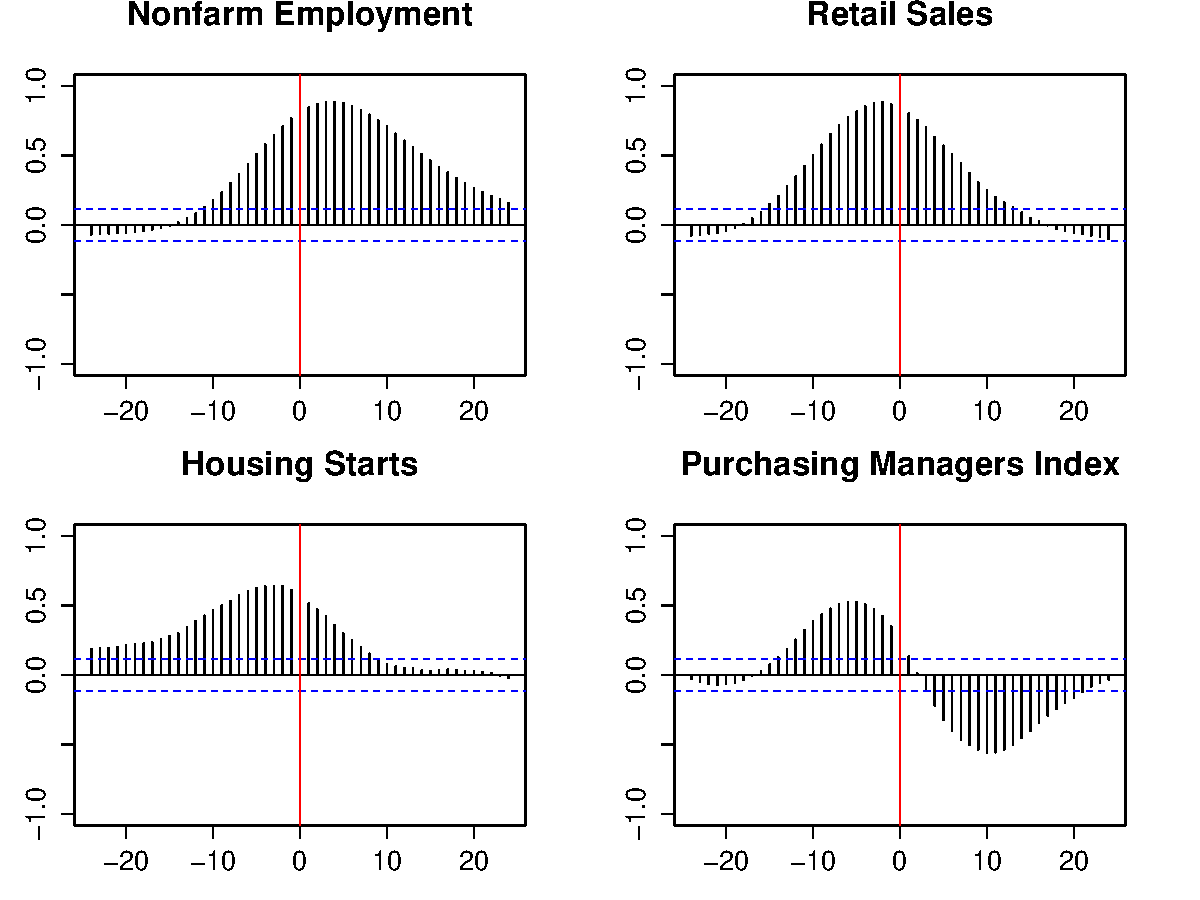
\includegraphics[width=0.85\textwidth]{ccf_plot.pdf}


Back to the question.  From the figure,
it seems that employment is a lagging indicator,
retails sales is leading, housing starts are leading (although the correlation is smaller
than for retails sales),
and the purchasing managers index is lagging
(the correlation to the right is larger in absolute value
than the correlation to the left, although you're free to use both).

For experts only:  The figure was computed in R, a popular open-source statistics program.
If you'd like to give it a try, save this pdf file, open it, and click on the pushpin:
\attachfile{ps3_f13.R} \\


\end{parts}
\end{solution}

% --------------------------------------------------------------------
\question {\it Near-term economic conditions (40 points).\/}
You are delighted to have a summer internship at JP Morgan.
Your first rotation:  the foreign exchange trading desk.
On your first day, the Managing Director gives you
a small project to get your feet wet.
Noting that currency markets are driven partly by macroeconomic news,
she asks you to write a report summarizing the near-term prospects for the US
economy, specifically the next two quarters.

You go (again) to FRED
and download 6-8 of your favorite economic indicators.
(If you're short of ideas, look at the Bloomberg
\href{http://www.bloomberg.com/markets/economic-calendar/}{economic calendar}
and the
\href{http://pages.stern.nyu.edu/~dbackus/macro_resources.htm}{resource page}.)
After collecting the data, you:
%
\begin{parts}
\part Explain (briefly) why you chose each indicator.
Comment also, if you like, on why you used the indicator,
its growth rate, or some other ``transformation.''
(10~points)

\part Graph each indicator (suitably transformed) over some sensible sample period.
What are the advantages of a long sample period?  Disadvantages?
Include on the graph lines representing
the sample mean and plus/minus one standard deviation.
(10~points)

\part Summarize your findings in a business cycle scorecard,
as outlined in the notes.
(10~points)

\part Overall, do they indicate above-average, below-average,
or average growth of the US economy?
What judgemental factors would you add to your analysis?
Where do you think the US economy is headed over the next 3-6 months?
(10~points)
\end{parts}

\begin{solution}
\begin{parts}
\item You'll have to use your own judgement here.
Part of the judgement involves which series to use.
Generally you want to use series whose ups and downs
are strongly correlated with those of the economy.
Another part is whether to use levels or growth rates.
Generally you want to use whatever works best;
unfortunately, there's no mechanical method to determine that.
With housing starts, for example, the growth rate looks pretty good right now,
but the level still looks bad.
Which is more informative?  Hard to say, we haven't been in this situation before.

\item Generally a long sample period has the advantage of giving us more data:
as a rule, the more data we have, the more precisely we can estimate patterns.
But if the world changes, then the risk with a long sample period is that the old data
does not represent current patterns.  
So there's a tradeoff.  
In the previous question we started in 1990, which seems like a reasonable compromise.  
We'll do the same here.  

The plot below includes three of the series (their growth rates, actually)
we looked at above with the requested lines added.

\begin{center}
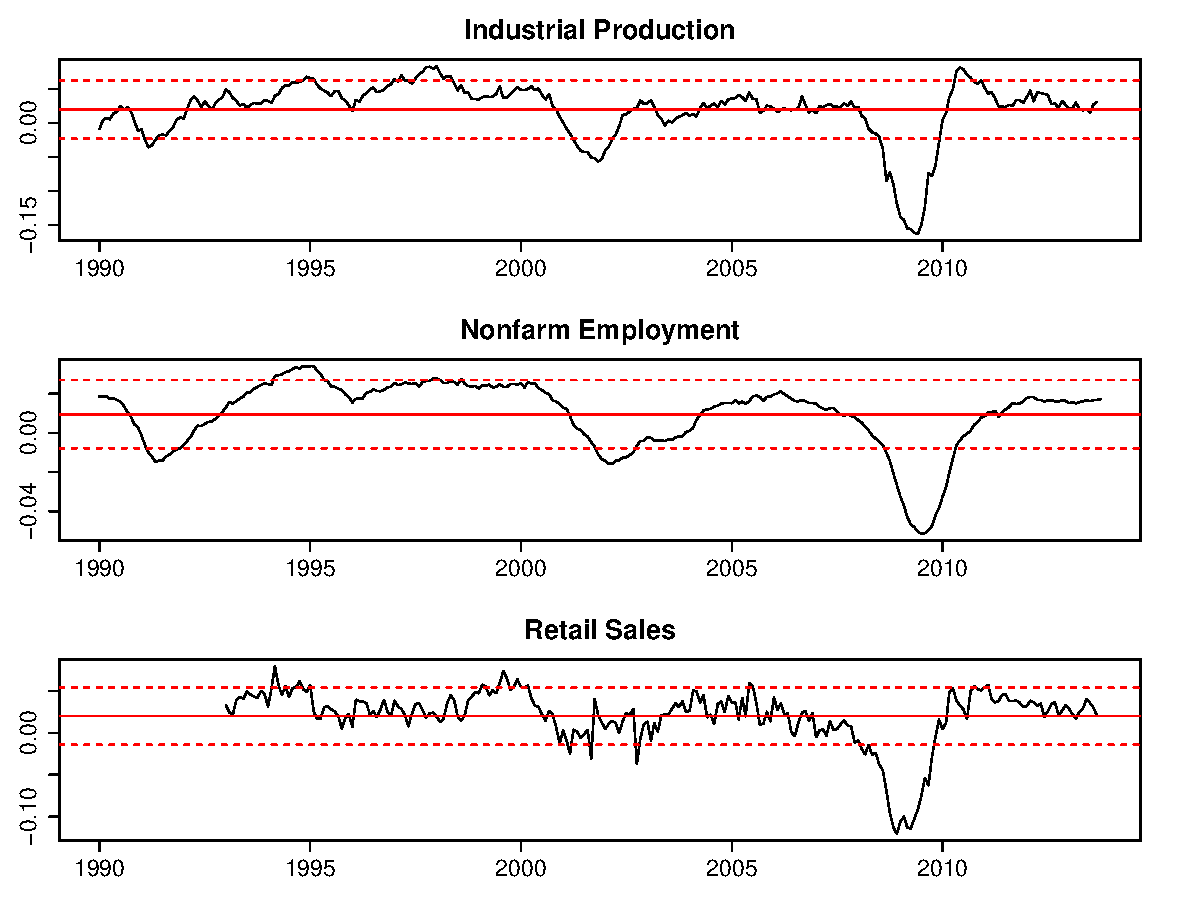
\includegraphics[width=0.85\textwidth]{scorecard.pdf}
\end{center}

\item In the figure above, all three indicators 
show up as weak positive:  above the mean, but below the mean
plus one standard deviation.  
In a business cycle scorecard, that would look like this:  

\begin{center}
\begin{tabular}{lcccc}
\toprule
            &  Strong    &  Weak  &  Weak   &  Strong  \\
Indicator   &  Negative  & Negative & Positive & Positive \\
\midrule
Industrial production  &&& x \\
Employment             &&  & x \\
Retail sales            & & & x \\
\midrule
Summary                & 0 & 0 & 3 & 0 \\
\bottomrule
\end{tabular}
\end{center}

\item Right now, most indicators seem to suggest average to slightly above average 
growth.  
That could easily change, but that's how it looks now.
As for the future:  
the leading indicators suggest the same, so the mainstream view is that 
the economy will continue to grow at a steady pace.

\end{parts}
\end{solution}

\end{questions}

\vfill \centerline{\it \copyright \ \number\year \
NYU Stern School of Business}

\end{document}

